\documentclass{standalone}
\usepackage{tikz}
%% \usepackage{pgfmath}

\begin{document}

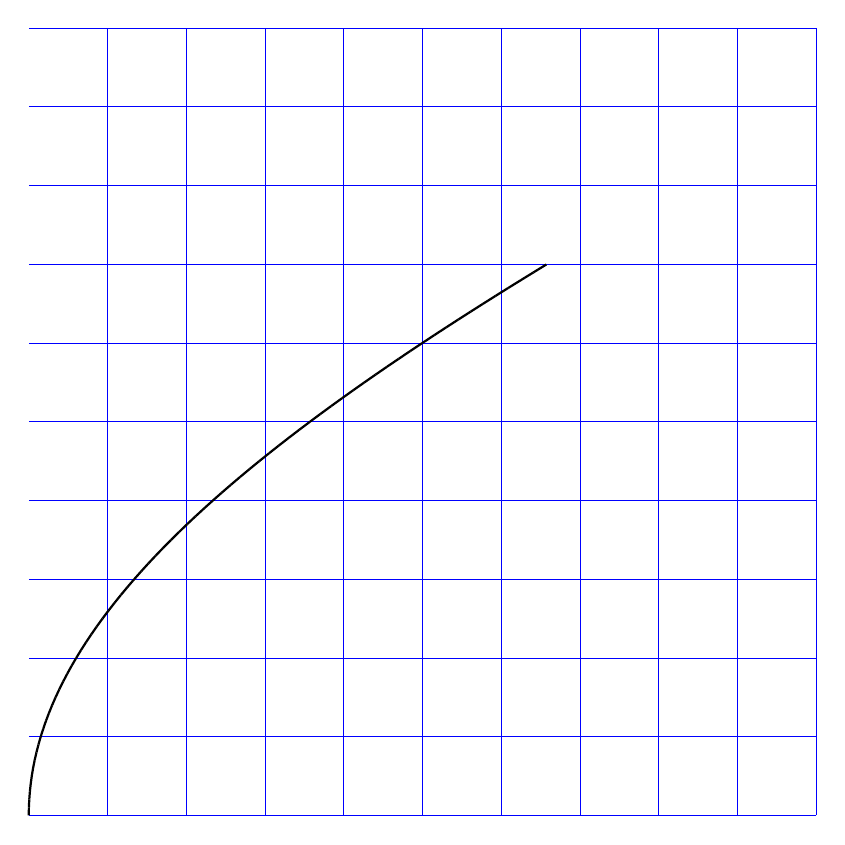
\begin{tikzpicture}[scale=10]
  \draw[blue,very thin, step=0.1cm] (-1,0) grid (0,1);
  \foreach \step in {0.60} { %for each of the curved lines
  %% \foreach \step in {0,2,...,10,20,30,40,50,60} { %for each of the curved lines
    \foreach \y in {0.0,0.01,...,0.69} {   %for each degree in the vertical scale
      \draw[thick]  ({(-sin(90-\y*100))},\y) -- ({(-sin(90-(\y+0.01)*100))},\y+0.01);
      %% \draw[thick] ({(sin(90-\y*100))*-\step},\y) -- ({(sin(90-(\y+0.01)*100))*-\step},\y-0.01);
    }
  }
  %% \foreach \lat in {0,10,...,70} {  %For each of the horizontal latitude lines
  %%   \draw[thick] ({sin(90-\lat)*-60+60},\lat) -- (60,\lat) node [right] {\lat};
  %% }
  %% \foreach \lat in {5,15,...,65} {  %For each of the thinner horizontal latitude lines
  %%   \draw[ very thin] (60,\lat) -- ({sin(90-\lat)*-60+60},\lat);
  %% }
  %% \foreach \min in {0,10,...,50} {     %For each minute in the latitude scale (skip 0)
  %%   \node [above left] at (50-\min, 0) {\min};
  %% }
\end{tikzpicture}

\end{document}
